
\chapter{The surface code}\label{ch:surfacecode}

The variant of the stabilizer codes that we are going to explore in this thesis is Kitaev's \emph{surface code} \cite{kitaev2003fault}, which is of the category of \emph{topological codes}. Among this category, the surface code is preferable as it offers the highest error tolerance under realise noise channels and requires only local stabilizer measurements of physically neighboring qubits. Two variants of the surface code will be considered here, the \emph{toric code} in Section \ref{sec:surface_toric} and the \emph{planar code} in Section \ref{sec:surface_planar}.
\begin{figure}[htbp]
    \centering
    \begin{tikzpicture}[scale=0.8]
      \DRAWTORIC{3}
      \draw [arrow] (-1,0 |- N-0-2-1) node [align=right, left] {qubit/edge} -- (N-0-2-1);
      \node (plaquette) at ($(N-0-1-0)!0.5!(N-0-0-0)$) {};
      \node (star) at ($(N-1-0-1)!0.5!(N-1-1-1)$) {};
      \draw [arrow] (-1,0 |- plaquette)  node [align=right, left] {face} -- (plaquette);
      \draw [arrow] (-1,0 |- N-1-0-1) node [align=right, left] {vertex} to [out=0, in=225] (star);
      \node [align=left, right] at (3*\s + .5, .5*\s) {periodic boundary};
  
    \end{tikzpicture}
    \caption{The toric code is defined as a $L\times L$ lattice (here $L=3$) with periodic boundary conditions. The edges on the lattice, which represents the qubits, make up faces and vertices (inspired by \cite{browne}).}\label{sf:fig_toriclattice}
  \end{figure}

\section{The toric code}\label{sec:surface_toric}
The \emph{toric code} is defined by arranging qubits on the edges of a square lattice with periodic boundary conditions, as seen in Figure \ref{sf:fig_toriclattice}. The name of the toric code lends itself from the torus, or doughnut, shape, where any point on the surface of the torus will encounter itself after traversing the torus in either x or y directions. Hence, the top edge of the toric code meets the bottom edge, whereas the left edge meets the right. On a $L\times L$ grid there are $n = 2L^2$ edges and the same amount of physical qubits. This topology of qubit arrangement plays an important part in encoding the logical qubits, which is stored in the non-trivial cycles on the torus. Errors, beneath a certain threshold, will only introduce local effects and does not change these cycles.

\subsection{Stabilizer generators}

To define a stabilizer code, we need to specify the $m$ independent stabilizer generators and the encoded $\hat{X}_L$ and $\hat{Z}_L$ operators. On the toric code there are two types of stabilizer generators, \emph{plaquette} and \emph{star} operators, which are associated with the \emph{faces} and \emph{vertices} of the square lattice, respectively.
\begin{figure}[htbp]
  \centering
  \begin{tikzpicture}
    \DRAWTORIC{3}
    \DRAWPLAQ{1}{1}
    \DRAWERROR{1}{1}{0}{z}
    \DRAWERROR{1}{1}{1}{z}
    \DRAWERROR{1}{0}{0}{z}
    \DRAWERROR{2}{1}{1}{z}
    \node[below of=Bx-1] {\emph{(a)}};
  \end{tikzpicture}
  \hspace{1cm}
  \begin{tikzpicture}
    \DRAWTORIC{3}
    \DRAWSTAR{1}{1}{3}
    \DRAWERROR{1}{1}{1}{x}
    \DRAWERROR{1}{1}{0}{x}
    \DRAWERROR{1}{2}{1}{x}
    \DRAWERROR{0}{1}{0}{x}
    \node[below of=Bx-1] {\emph{(b)}};
  \end{tikzpicture}

  \begin{center}
    \hspace{1cm}
    \begin{tikzcd}[row sep={0.5cm,between origins}]
      \lstick{$Q_1$} & \qw & \qw & \qw & \ctrl{5} & \qw \\
      \lstick{$Q_2$}& \qw & \qw & \ctrl{4} & \qw & \qw \\
      \lstick{$Q_3$} & \qw & \ctrl{3} & \qw & \qw & \qw \\
      \lstick{$Q_4$} & \ctrl{2} & \qw & \qw & \qw & \qw \\
      &&&&&&&\\
      \lstick{$\hat{P}_f$} & \ctrl{} & \ctrl{} & \ctrl{} & \ctrl{} & \meter{}
    \end{tikzcd}
    \begin{tikzcd}[row sep={0.5cm,between origins}]
      \lstick{$Q_1$} & \qw & \qw & \qw & \targ{} & \qw \\
      \lstick{$Q_2$} & \qw & \qw & \targ{} & \qw & \qw \\
      \lstick{$Q_3$} & \qw & \targ{} & \qw & \qw & \qw \\
      \lstick{$Q_4$} & \targ{} & \qw & \qw & \qw & \qw \\
      &&&&&&&\\
      \lstick{$\hat{S}_v$} & \ctrl{-2} & \ctrl{-3} & \ctrl{-4} & \ctrl{-5} & \meter{}
    \end{tikzcd}
  \end{center}

  \caption{Each face (a) and vertex (b) on the lattice represents a plaquette and star operator. The non-identity single qubit operators on which they act are indicated by the Pauli operators. The set of all products of plaquette and star operators make up the stabilizers of the code. This figure is inspired by others  \cite{browne}.}\label{sf:fig_stabilizers}
\end{figure}

\begin{definition}
  A plaquette operator $\hat{P}_f$ consists of the tensor product of Pauli Z operators on qubits on the edges connected to a face $f$ (see Figure \ref{sf:fig_toriclattice}a,
  \begin{equation}\label{eq:sf_plaquette}
    \gls{oplaquette} = \prod_{i\in Q(f)} \hat{Z}_i
  \end{equation}
  where $Q(f)$ is the set of qubits touching face $f$. On a $L\times L$ grid there are $L^2$ plaquettes.
\end{definition}

\begin{definition}
  A star operator $\hat{S}_v$ consists of the tensor product of Pauli X operators on qubits neighboring the vertex $v$ (see Figure \ref{sf:fig_toriclattice}b,
  \begin{equation}\label{eq:sf_star}
    \gls{ostar} = \prod_{i\in Q(v)} \hat{X}_i
  \end{equation}
  where $Q(v)$ is the set of qubits neighboring vertex $v$. On a $L\times L$ grid there are $L^2$ plaquettes.
\end{definition}

As each plaquette and star operator needs to be measured, an ancilla qubit is needed at the physical locations of each of these operators. The structure of the full lattice is now clear, as it just a simple square arrangement of alternating data and ancilla qubits in both x and y directions.

The full stabilizer of the code $\m{S}$ can be generated by multiplying elements of the generator operators (see Definition \ref{def:stabilizer}). Consider two plaquette operators. These two operators will either share one boundary consisting of a qubit, or none. This means that the Pauli Z operator on the boundary qubit will add up to identity as they commute. The result is that the product of the plaquette operators will consists of the overall boundary Pauli operators of the joint plaquette (see Figure \ref{sf:fig_multistab}a.

However, if all plaquettes are applied to the lattice, no boundary will be left. Thus the product of all plaquettes is the identity, which means that the full set of plaquettes are not independent. The full set of plaquette generators can therefore be completed by simply removing a single plaquette from all available plaquettes. There are therefore $L^2 - 1$ independent plaquette operators.

The multiplication of star operators follow the same properties as the plaquette operators described above (see Figure \ref{sf:fig_multistab}b. Thus there are also $L^2 - 1$ independent star operators, which are the star generators. This sums up to $n_S = 2L^2 - 2$ independent stabilizer generators.

\begin{figure}[htbp]
  \centering
  \begin{tikzpicture}
    \DRAWTORIC{3}
    \DRAWPLAQ{1}{1}
    \DRAWPLAQ{0}{1}
    \DRAWPLAQ{0}{2}
    \DRAWERROR{1}{1}{0}{z}
    \DRAWERROR{1}{0}{0}{z}
    \DRAWERROR{2}{1}{1}{z}
    \DRAWERROR{0}{0}{0}{z}
    \DRAWERROR{0}{1}{1}{z}
    \DRAWERROR{0}{2}{1}{z}
    \DRAWERROR{0}{2}{0}{z}
    \DRAWERROR{1}{2}{1}{z}
    \node[below of=Bx-1] {(a)};
  \end{tikzpicture}
  \hspace{1cm}
  \begin{tikzpicture}
    \DRAWTORIC{3}
    \DRAWSTAR{1}{1}{3}
    \DRAWSTAR{2}{0}{3}
    \DRAWSTAR{2}{1}{3}
    \DRAWERROR{1}{2}{1}{x}
    \DRAWERROR{0}{1}{0}{x}
    \DRAWERROR{2}{2}{1}{x}
    \DRAWERROR{1}{1}{1}{x}
    \DRAWERROR{1}{0}{0}{x}
    \DRAWERROR{2}{0}{1}{x}
    \DRAWERROR{2}{0}{0}{x}
    \DRAWERROR{2}{1}{0}{x}
    \node[below of=Bx-1] {(b)};
  \end{tikzpicture}
  \caption{Multiplication of (a) plaquette and (b) star operators will result in a operator that consists of the Pauli operators that reside on the overall boundary of the joint plaquettes or stars (inspired by \cite{browne}).}\label{sf:fig_multistab}
\end{figure}

\subsection{Dual lattice}
Note that if we shift our lattice half a cell down, and half a cell to the right, we can create a \emph{dual} lattice. This dual lattice has the same size and same boundary conditions as the \emph{primal} lattice, but every plaquette in the primal lattice is a star in the dual lattice, and every star in the primal lattice is a plaquette in the dual lattice. The edges of the dual lattice are plotted with dotted lines in the figures.

This interesting property of \emph{lattice duality} leads to the fact that plaquette and star operators are in fact the same, and we can choose from either that is best suited for the calculation. The multiplication of operators is best pictured in the plaquette picture, for example. For the square lattice in the toric code, the dual lattice is coincidentally also square. For other types of topological codes with non-square lattices, the dual lattice has a different lattice structure than the primal lattice. We will not explore these kind of lattices in this thesis.

\subsection{Encoded qubits}
Since there are $n = L^2$ qubits and $n_S = 2L^2 - 2$ independent stabilizers, we must have $n_L = n - n_S = 2$ encoded qubits and therefore 4 logical operators $\hat{X}_{L1}, \hat{X}_{L2}, \hat{Z}_{L1}$ and $\hat{Z}_{L2}$.

Recall the logical operators consists of the Pauli operators, and must commute with all stabilizer generators, but cannot be part of the stabilizer itself. We can construct the logical operators by starting with, for example, a single Pauli Z operator. It commutes with all plaquette operators trivially. In terms of the star operators, this single Pauli Z operator commutes with all but the two neighboring qubits, as all others apply to different qubits. Adding another Pauli Z operator will shift will of the neighboring star operators that anticommute. We know see that a closed loop of Z operators around the torus does not have neighboring star operators, and therefore commute with all stabilizers. As the torus has two directions we can loop over, these are the logical $\hat{Z}_L$ operators (see Figure \ref{sf:fig_logical}a-b). Analogously, we can construct the logical $\hat{X}_L$ operators in the same way (Figure \ref{sf:fig_logical}c-d).

Note that these logical operators are not unique. As the logical operators commute with the stabilizers, these $\hat{X}_L$ and $\hat{Z}_L$ operators can be multiplied with e.g.\ a plaquette or star operator, respectively, which create a diversion from its original path. But as the path still loops around the torus, this is still a valid logical operator.

The logical operators have a minimum length of $L$ qubits, which is also the distance of the toric code (see Definition \ref{def:distance}). The toric code is therefore a $[L^2,2,L]$ in the [n,k,d] notation. This implies that the toric code might be more robust against errors if the size of the lattice is increased. Later we will see that this is also very much dependent on the type of decoder that is used, and that different decoders will lead to different regimes of error for which this reasoning is true.
\def\QS{10}
\def\s{1}

\begin{figure}[htbp]
  \centering
  \begin{tikzpicture}
    \DRAWTORIC{5}
    \DRAWERROR{0}{2}{0}{z}
    \DRAWERROR{1}{2}{0}{z}
    \DRAWERROR{2}{2}{0}{z}
    \DRAWERROR{3}{2}{0}{z}
    \DRAWERROR{4}{2}{0}{z}
    \DRAWERROR{3}{0}{1}{z}
    \DRAWERROR{3}{1}{1}{z}
    \DRAWERROR{3}{2}{1}{z}
    \DRAWERROR{3}{3}{1}{z}
    \DRAWERROR{3}{4}{1}{z}
    \begin{pgfonlayer}{edges}
      \draw[synz] (S-0-2) -- (S-5-2);
      \draw[synz] (S-3-4) -- (S-3-5);
    \end{pgfonlayer}
    \node[above=.25cm of S-3-4] {(a)};
    \node[left=.25cm of S-0-2] {(b)};
  \end{tikzpicture}
  \hspace{1cm}
  \begin{tikzpicture}
    \DRAWTORIC{5}
    \DRAWERROR{0}{2}{1}{x}
    \DRAWERROR{1}{2}{1}{x}
    \DRAWERROR{2}{2}{1}{x}
    \DRAWERROR{3}{2}{1}{x}
    \DRAWERROR{4}{2}{1}{x}
    \DRAWERROR{3}{0}{0}{x}
    \DRAWERROR{3}{1}{0}{x}
    \DRAWERROR{3}{2}{0}{x}
    \DRAWERROR{3}{3}{0}{x}
    \DRAWERROR{3}{4}{0}{x}
    \begin{pgfonlayer}{edges}
      \draw[synx] (N-0-2-1) -- (By-2);
      \draw[synx] (Bx-3) -- (N-3-4-0);
    \end{pgfonlayer}
    \node[above=.25cm of N-3-4-0] {(c)};
    \node[right=.25cm of By-2] {(d)};
  \end{tikzpicture}
  \caption{The logical (a) $\hat{X}_{L1}$, (b) $\hat{X}_{L2}$, (c) $\hat{Z}_{L1}$ and (d) $\hat{Z}_{L2}$ operators are the closed loop of $X$ and $Z$ operators, respectively, that go around the two boundaries of the torus (inspired by \cite{browne}).}\label{sf:fig_logical}
\end{figure}


\subsection{Error detection}
As discussed in the previous chapter, errors are detected by measuring the set of stabilizer generators. As we have seen in the previous section, this consists of all but one plaquette operators $\hat{P}_f$ and all but one star operators $\hat{S}_v$. Let us first consider to measure all of them.

In the case of a single Z-error (Fig \ref{sf:fig_degenerate}a.i), the neighboring plaquette operators will commute with this error, as it consists of Pauli Z operators itself. But the neighboring star operators anticommutes with this error according to equation \eqref{qec:eq:stabmeas}. Similarly, a single X-error (Fig \ref{sf:fig_degenerate}a.ii) commutes with neighboring star operators but anticommutes with neighboring plaquette operators. An Y-error is a combination of X and Z operators and therefore anticommutes with all neighboring generator operators (Fig \ref{sf:fig_degenerate}a.iii).

In the case of two Z-errors (Fig \ref{sf:fig_degenerate}a.iv), the star operators between the two errors now commute with the errors, creating a virtual path between them. This is a general property: given any string of errors, the generator operators at the end of the string will anticommute with the errors and measure -1. For Z-errors, star operators at the end of strings on the primal lattice will measure -1. The detection of X-errors occur in the same way, albeit now the strings of errors is defined on the \emph{dual} lattice, and plaquette errors will measure -1 at the end of these strings.

Since Z and X-errors independently affect different types of stabilizer measurements (stars and plaquettes, respectively), these two types of errors can be considered independently in two error correction processes. The two processes are analogous, up to the duality of the lattice. Therefore, for the remainder of the section, only Z-errors, which leave a string of errors on the primal lattice, will be considered.

\begin{figure}[htbp]
    \centering
    \begin{tikzpicture}
      \DRAWTORIC{5}
      \DRAWERROR{1}{2}{0}{z}
      \DRAWERROR{2}{4}{1}{x}
      \DRAWERROR{3}{1}{0}{y}
      \DRAWERROR{1}{0}{0}{z}
      \DRAWERROR{0}{0}{0}{z}
      \DRAWPLAQ{1}{4}
      \DRAWPLAQ{2}{4}
      \DRAWSTAR{1}{2}{5}
      \DRAWSTAR{2}{2}{5}
      \DRAWSTAR{0}{0}{5}
      \DRAWSTAR{2}{0}{5}
      \DRAWPLAQ{3}{1}
      \DRAWPLAQ{3}{2}
      \DRAWSTAR{3}{1}{5}
      \DRAWSTAR{4}{1}{5}
      \begin{pgfonlayer}{edges}
        \draw[synz] (N-0-0-0) -- (N-1-0-0);
      \end{pgfonlayer}
      \node[below=.25cm of Bx-2] {(a)};
      \node[script] at (P-1-2) {\textit{(i)}};
      \node[script] at (P-1-4) {\textit{(ii)}};
      \node[script] at (P-3-1) {\textit{(iii)}};
      \node[script] at (P-1-0) {\textit{(iv)}};
  
    \end{tikzpicture}
    \hspace{1cm}
    \begin{tikzpicture}
      \DRAWTORIC{5}
      \DRAWERROR{0}{2}{0}{z}
      \DRAWERROR{2}{2}{0}{z}
      \DRAWERROR{3}{2}{0}{z}
      \DRAWERROR{4}{2}{0}{z}
      \DRAWSTAR{1}{2}{5}
      \DRAWSTAR{2}{2}{5}
      \begin{pgfonlayer}{edges}
        \draw[synz] (N-0-2-0) -- (S-0-2) (N-2-2-0) -- (S-5-2);
      \end{pgfonlayer}
      \node[below=.25cm of Bx-2] {(b)};
    \end{tikzpicture}
  
    \begin{tikzpicture}
      \DRAWTORIC{5}
      \DRAWERROR{1}{2}{1}{z}
      \DRAWERROR{1}{1}{1}{z}
      \DRAWERROR{1}{0}{0}{z}
      \DRAWERROR{2}{0}{1}{z}
      \DRAWERROR{2}{4}{1}{z}
      \DRAWERROR{2}{3}{1}{z}
      \DRAWSTAR{1}{2}{5}
      \DRAWSTAR{2}{2}{5}
      \begin{pgfonlayer}{edges}
        \draw[synz] (N-1-2-1) -- (S-1-0) -- (S-2-0) -- (S-2-5) (S-2-4) -- (N-2-3-1);
      \end{pgfonlayer}
      \node[below=.25cm of Bx-2] {(c)};
    \end{tikzpicture}
    \hspace{1cm}
    \begin{tikzpicture}
      \DRAWTORIC{5}
      \DRAWERROR{0}{2}{0}{z}
      \DRAWERROR{4}{2}{0}{z}
      \DRAWERROR{4}{2}{1}{z}
      \DRAWERROR{4}{1}{1}{z}
      \DRAWERROR{3}{0}{0}{z}
      \DRAWERROR{3}{0}{1}{z}
      \DRAWERROR{3}{4}{1}{z}
      \DRAWERROR{3}{3}{1}{z}
      \DRAWERROR{2}{2}{0}{z}
      \DRAWSTAR{1}{2}{5}
      \DRAWSTAR{2}{2}{5}
      \begin{pgfonlayer}{edges}
        \draw[synz] (N-0-2-0) -- (S-0-2) (N-2-2-0) -- (S-3-2) -- (S-3-4);
        \draw[synz] (S-3-5) -- (S-3-0) -- (S-4-0) -- (S-4-2) -- (S-5-2);
      \end{pgfonlayer}
      \node[below=.25cm of Bx-2] {(d)};
    \end{tikzpicture}
    \caption{(a) Stabilizer generators that anticommute with the error will measure -1, which are (i) the neighboring star operators for a Z-error, (ii) the neighboring plaquette operators for an X-error, and (iii) both star and plaquette operators for a Y-error. In the case of a string of errors (iv), only the stabilizer generators at the end of these strings will anticommute with the error. Due to code degeneracy, the single Z-error in (a.i) $\hat{E}$ has the syndrome as (b) $\hat{E}\hat{Z}_{L1}$, (c) $\hat{E}\hat{Z}_{L2}$ and (d) $\hat{E}\hat{Z}_{L1}\hat{Z}_{L2}$ (inspired by \cite{browne}).}\label{sf:fig_degenerate}
  \end{figure}

\subsection{Error correction}\label{sec:correction}
An error can be corrected by applying it again to the lattice. However, the problem is that the error operator $\hat{E}$ is unknown. We must therefore try to identify the correct operator given the measured syndrome. As mentioned in the previous chapter, this relationship between error does not always map one-to-one, which it is not in the surface code. An error $\hat{E}$ can be multiplied with some operator $L$ that commutes with the stabilizer, and they will result in the same syndrome.

If $\hat{L}$ is in the stabilizer $\m{S}$, the product of the identified correction operator $\gls{ocorrection}=\hat{E}'$ with the real error operator $\hat{E}$ will leave the code invariant. The resulting operator $\hat{C}\hat{E}\hat{L}$ is a stabilizer operator $\hat{S}$. However, the encoded logical operators also commute with the stabilizer, which means that $\hat{E}$, $\hat{E}\hat{Z}_{L1}$, $\hat{E}\hat{Z}_{L2}$, $\hat{E}\hat{Z}_{L1}\hat{Z}_{L2}$ will all lead to the same syndrome (Fig \ref{sf:fig_degenerate}a-d). Any identified correction operator $\hat{C}$ can therefore be categorized into four classes of operators, of which only one includes the correct logical operator. The task of choosing most appropriate correction chain is up to the decoders.

\subsection{Decoding}\label{sec:threshold}
Since the distance $d$ of the toric code on a $L\times L$ is $L$, we would expect that we can improve the robustness of the code by increasing the lattice size $L$. However, this also increases the total number of errors in the lattice, that adds an increased level of complexity in choosing the correct correction operator.

In practice, there is a trade-off between the positive effect of a larger code distance and the negative effect of larger number of errors. When the error rate $p$ is low, the positive effect outweighs the negative and increasing the lattice $L$ will increase the probability of successful error correction $\gls{zpcorrect}$. When the error rate is large, the negative effect outweighs the positive and increasing $p$ will decrease $k_C$. The point of transition in the error rate is called the \emph{code threshold} $\gls{zpthres}$.

The code threshold is not the only parameter that determines the potential of a certain code for practical use. The behavior for error rates far below the threshold is also important, as is the number of physical qubits needed to achieve the sought after level of error suppression. Nevertheless, the code threshold provides us with a very easy and useful tool to benchmark different codes and different decoding algorithms, and to compare them with each other. Therefore, in this thesis we will heavily rely on the value of the code threshold. The value of the threshold is heavily dependent on the chosen error model and the physical conditions of the stabilizer measurements. To compare different decoding algorithms, we therefore will use independent and identically distributed errors (i.i.d. noise), which is the \emph{independent noise model} from Section \ref{qec:sec_errormodels}.

\todo[inline]{Nishimori, optimal value}

For the toric code, when the only source of errors is i.i.d. noise under the independent noise model, and all measurements can be made perfectly, the \emph{optimal threshold} has been proven to be 10.9\%. However, to achieve this value, one needs to consider all possible error configurations on the lattice to identify the correction operator $C$ that is most likely to be equal to the error operator $E$. This is a computationally heavy task that scales exponentially with the lattice size. It is therefore an impractical approach in reality.

Luckily, there exists other decoding algorithms that can find a solution much faster, albeit at the cost of reducing the code threshold. Edmond's \emph{Minimum Weight Perfect Matching} decoder scales cubic with the system, which allows for faster decoding, and achieves a code threshold of 10.3\% (Chapter \ref{ch:mwpm}). Including faulty measurements the threshold drops down to 2.9\%. The \emph{Union-Find} decoder is a relatively new addition to the set of decoders for the surface code. It scales \emph{almost} linearly with the system, and has a code threshold of 9.9\% (Chapter \ref{ch:UFdecoder}). In this thesis, we will try to combine certain properties of different decoders. In particular, we have created a heuristic for minimum weight which can be applied to the Union-Find decoder.


\subsection{Quasiparticle picture}\label{sec:quasiparticle}
The processes of error detection and correction can alternatively be presented in the \emph{quasiparticle picture}, where the anticommuting stabilizer measurements act like excitations on the lattice, which behave like the quasiparticles \emph{anyons}. A single error creates a pair of anyons, and a chain of errors causes movement of the anyon on the lattice. A pair of anyons can also annihilate each other when two error chains merge. The correction of errors can thus be viewed of movement of the correction chains until all anyons are annihilated. The quasiparticle picture removes the distracting underlying lattice from the problem, and decoding becomes simply identifying the right pairing between anyons to minimize the chance of a logical error.
\tikzstyle{rednode}=[circle, fill=red!50, minimum size=4]
\tikzstyle{bluenode}=[circle, fill=cyan!50, minimum size=4]
\tikzstyle{redline}=[red!50, line width = 2]
\tikzstyle{blueline}=[cyan!50, line width = 2]

\newcommand{\drawquasigrid}{
  \draw[step=.4cm, opacity=.25] (0,0) grid (4,4);
  \draw (0,0) rectangle (4,4);
  \node[rednode] (N1) at (0.5,0.4) {};
  \node[rednode] (N2) at (2,0.7) {};
  \node[rednode] (N3) at (2.5,1.2) {};
  \node[rednode] (N4) at (3.6,1) {};
  \node[rednode] (N5) at (0.75,2.1) {};
  \node[rednode] (N6) at (1.95,1.8) {};
  \node[bluenode] (N7) at (1.6, 3.4) {};
  \node[bluenode] (N8) at (2.7, 3.5) {};
  \node[bluenode] (N9) at (3.2, 1.5) {};
  \node[bluenode] (N10) at (3.1, 0.6) {};
  \draw[blueline] (N1) to[in=170, out=20] (N2);
  \draw[blueline] (N3) to[in=180, out=-10] (N4);
  \draw[blueline] (N5) to[in=170, out=-20] (N6);
  \draw[redline] (N7) to[in=160, out=15] (N8);
  \draw[redline] (N9) to[in=90, out=250] (N10);
}
\begin{figure}
    \centering
    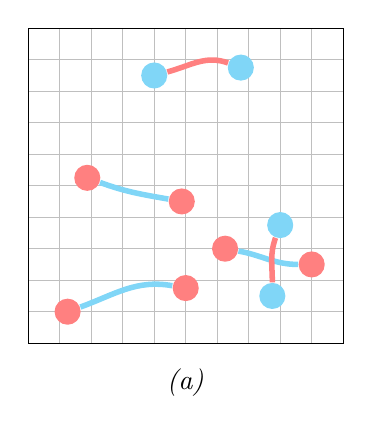
\begin{tikzpicture}
      \drawquasigrid
      \node at (2, -.5) {\emph{(a)}};
    \end{tikzpicture}
    \hspace{1cm}
    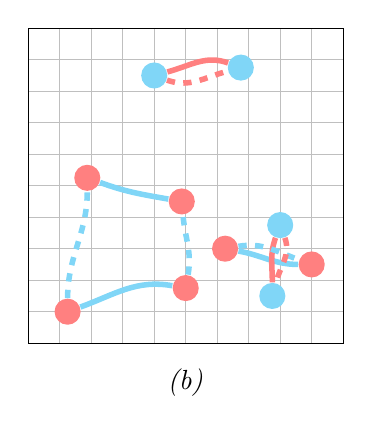
\begin{tikzpicture}
      \drawquasigrid
      \draw[dashed, blueline] (N1) to[out=90, in=270] (N5);
      \draw[dashed, blueline] (N2) to[out=80, in=275] (N6);
      \draw[dashed, blueline] (N3) to[out=10, in=160] (N4);
      \draw[dashed, redline] (N7) to[out=-20, in=195] (N8);
      \draw[dashed, redline] (N9) to[out=290, in=75] (N10);
      \node at (2, -.5) {\emph{(b)}};
    \end{tikzpicture}
    \hspace{1cm}
    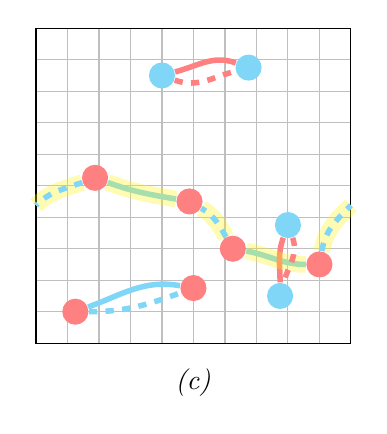
\begin{tikzpicture}
      \drawquasigrid
      \draw[yellow, line width=6, opacity=.3] (N3) to[in=180, out=-10] (N4);
      \draw[yellow, line width=6, opacity=.3] (N5) to[in=170, out=-20] (N6);
      \draw[yellow, line width=6, opacity=.3] (N3) to[out=120, in=-30] (N6);
      \draw[yellow, line width=6, opacity=.3] (N5) to[out=200, in=45] (0, 1.75);
      \draw[yellow, line width=6, opacity=.3] (N4) to[out=80, in=225] (4, 1.75);
      \draw[dashed, blueline] (N1) to[out=0, in=200] (N2);
      \draw[dashed, blueline] (N3) to[out=120, in=-30] (N6);
      \draw[dashed, blueline] (N5) to[out=200, in=45] (0, 1.75);
      \draw[dashed, blueline] (N4) to[out=80, in=225] (4, 1.75);
      \draw[dashed, redline] (N7) to[out=-20, in=195] (N8);
      \draw[dashed, redline] (N9) to[out=290, in=75] (N10);
      \node at (2, -.5) {\emph{(c)}};
    \end{tikzpicture}
    \caption{The quasiparticle picture of stabilizer measurements. Anticommuting stabilizers behave as anyons (circles), where a chain of errors (lines) creates a pair of anyons. Figure (b) shows a successful decoding of (a). Figure (c) shows a pairing that resulted in a correction operator that is in a different class as the error operator, which acquires a logical error. (Figure inspired by \cite{naomi})}\label{fig:quasiparticle}
  \end{figure}
  

Figure \ref{fig:quasiparticle}a shows the quasiparticle representation of the errors suffered in Figure \ref{sf:fig_degenerate}a, which has suffered Z (blue lines) and X errors (red lines). The corresponding anyons can either be of the star type (red circle) or plaquette type (blue circle). Figure \ref{fig:quasiparticle}b shows a successful decoding. Note that here not all pairs are correctly identified, but the resulting loop still is in the same class of operators. In Figure \ref{fig:quasiparticle}c the correction has failed as the resulting loop in the correction is in a difference class compared to the error. As the loop still commutes with the stabilizer, no error can be detected, but the encoded qubit has acquired a logical error.


\subsection{Graph picture}\label{sec:toricgraph}
Since it is the combinatorial structure of the lattice that defines the surface code, such a surface by be also denoted by a graph $\gls{ngraph}$. The graph is constructed by $G(\gls{svertices}, \gls{sedges}, \gls{sfaces})$ by a vertex set $\m{V}$, edge set $\m{E}$ and face set $\m{A}$. Each edge $\gls{nedge}\in \m{E}$ is defined by a pair of distinct vertices $e=\{v_i, v_j\}$ where $\gls{nvertex}\in \m{V}$. Each face is a region that has the homology of a disk and is defined by the set of edges on its boundary. 

With respect to the toric code, each vertex refers to a ancillary qubit corresponding to a star operator $v\equiv \hat{S}_v$, and each face $\gls{nface}\in \m{A}$ refers to a ancillary qubit corresponding to a plaquette operator $f\equiv \hat{P}_f$. The edges are thus the qubits, with two edges per qubit, one spanned by neighboring vertices and another by neighboring faces. Due to the duality of the lattice, the equivalence of vertices with stars and faces with plaquettes can naturally be switched. Also due to this, the graph $G$ can be split into two separate graphs $G_v(\m{V}, \m{E}_v)$ and $\m{G}_v(\m{A}, \m{E}_v)$, corresponding to the primal and dual lattices, where $E_v$ are the edges connecting the vertices $\m{V}$, and $\m{E}_f$ are the edges connecting the faces $\m{A}$. Each qubit is now represented by a single edge in both graphs and $\m{E}_v\cup \m{E}_f=\m{E}$. If we mention a graph spanned by only vertices and edges $(\m{V},\m{E})$, we refer to the graph $G_v$ of the primal lattice. 

\section{The planar code}\label{sec:surface_planar}
Another variant of the surface code is the \emph{planar code}, which disposes the periodic boundary conditions of the torus. This allows the qubits to be placed onto a flat 2D surface. For real systems in which the qubits physically interact with each other, this is a huge benefit. Therefore, in this thesis, we will consider both toric and planar variants of the surface code.

\def\QS{15}
\def\s{1.5}
\begin{figure}[htbp]
  \centering
  \begin{tikzpicture}
    \DRAWPLANAR{6}
    \DRAWPLAQ{1}{3}
    \DRAWEPLAQ{0}{5}
    \DRAWSTAR{3}{3}{4}
    \DRAWESTAR{2}{5}
    \DRAWERROR{1}{3}{0}{z}
    \DRAWERROR{1}{3}{1}{z}
    \DRAWERROR{1}{2}{0}{z}
    \DRAWERROR{2}{3}{1}{z}
    \DRAWERROR{0}{4}{0}{z}
    \DRAWERROR{0}{5}{0}{z}
    \DRAWERROR{1}{5}{1}{z}
    \DRAWERROR{1}{5}{0}{x}
    \DRAWERROR{2}{5}{0}{x}
    \DRAWERROR{2}{5}{1}{x}
    \DRAWERROR{2}{3}{0}{x}
    \DRAWERROR{3}{3}{0}{x}
    \DRAWERROR{3}{3}{1}{x}
    \DRAWERROR{3}{4}{1}{x}
    \DRAWERROR{4}{0}{0}{x}
    \DRAWERROR{4}{1}{0}{y}
    \DRAWERROR{4}{2}{0}{x}
    \DRAWERROR{4}{3}{0}{x}
    \DRAWERROR{4}{4}{0}{x}
    \DRAWERROR{4}{5}{0}{x}
    \DRAWERROR{0}{1}{0}{z}
    \DRAWERROR{1}{1}{0}{z}
    \DRAWERROR{2}{1}{0}{z}
    \DRAWERROR{3}{1}{0}{z}
    \DRAWERROR{5}{1}{0}{z}
    \begin{pgfonlayer}{edges}
      \draw[synz] (N-0-1-0) -- (N-5-1-0);
      \draw[synx] (N-4-5-0) -- (N-4-0-0);
    \end{pgfonlayer}
    \node[script] at (P-1-3) {(c)};
    \node[script] at (S-3-3) {(d)};
    \node[script] at (P-0-5) {(a)};
    \node[script] at (S-2-5) {(b)};
    \node[above=.25cm of N-4-5-0] {(f)};
    \node[left=.25cm of N-0-1-0] {(e)};
  \end{tikzpicture}
  \caption{The planar code with lattice size $L=4$, which includes $n = 2L^2-2L+1$ qubits and $n_S = 2L^2-2L$ independent stabilizers. The boundary is defined by the (a) $\delta$-plaquette and (b) $\delta$-star operators, which exist next to the known (c) plaquette and (d) star operators, similar to the toric code. The planar codes encodes 1 logical qubit, which is represented by the logical (e) $\hat{Z}_L$ and (f) $\hat{X}_L$ operators (inspired by \cite{browne}).}\label{sf:fig_planar}
\end{figure}

\paragraph{Stabilizer generators}
There are a few key differences between the planar and toric codes. First of all, a new type of stabilizer generators define the non-periodic boundary of the lattice, which are referred to as \emph{$\delta$ operators}. These $\delta$ operators have only 3 neighboring qubits and are therefore the tensor product of 3 Pauli operators. The $\delta$-plaquette operators lie at the east and west boundaries of the lattice (Figure \ref{sf:fig_planar}a and the $\delta$-star operators lie at the north and south boundaries of the lattice (Figure \ref{sf:fig_planar}b. In the middle of the lattice, the bulk of the stabilizer generators still consist of 4 Pauli operators, identical to the ones in the toric code (Figure \ref{sf:fig_planar}c-d). Note that the stabilizer generators are still defined by equation \eqref{eq:sf_plaquette} and \eqref{eq:sf_star}, but now the relevant faces and vertices contain three neighboring qubits.

\paragraph{Stabilizer violoations}
A second key difference is that now not all errors will cause two stabilizer violations. In the bulk of the qubits on the lattice, a single error will still cause two neighboring stabilizers to measure -1, or create two anyons. At the boundary however, it now may be the case that an error is only included in one plaquette or star operator. This will also mean the decoding in the quasiparticle picture requires a slightly different approach.

\paragraph{Encoded qubits}
Furthermore, we can inspect that a planar surface of dimension $L$ has $n = 2L^2-2L+1$ physical qubits. We can also find that there are $2L^2-2L$ stabilizer generators. As the boundary is now non-periodic, all generators are now independent, and therefore the number independent generators is $n_S = 2L^2-2L$. This means that the planar code encodes $n_L = n-n_S = 1$ a single logical qubit. The logical $\hat{X}_L$ and $\hat{Z}_L$ operators are pictured in Figure \ref{sf:fig_planar}e-f.

\paragraph{Dual lattice and graph picture}
Other properties of the planar code are very similar to the toric code. The \emph{dual lattice} also exists for the planar code, for example. But the dual lattice exists at a 90 angle compared to the primal lattice to account for the location of the boundary. The elements of the graph $G(\m{V},\m{E},\m{A})$ can now be separated into disjoint subsets due to the different properties of its vertices, edges and faces. The vertex set $\m{V}$ can now be divided into; the internal vertex set $\m{V}_\iota$ consisting of 4-Pauli-operator stabilizers; the boundary vertex set $\m{V}_{\delta}$ consisting of 3-Pauli-operator stabilizers; and the open vertex set $\m{V}_\omega$ consisting of non-stabilizer vertices that span edges on the boundary $\m{E}_{\delta}$ that connected to a single stabilizer vertex. Note that vertices of $\m{V}_\omega$ thus do not correspond to any physical stabilizer measurements. Edges connected to two stabilizer vertices belong to the internal edge set $\m{E}_\iota$. The graph for the primal lattice is hence $G(\m{V}_\iota\cup \m{V}_\delta \cup \m{V}_\omega, \m{E}_\iota\cup \m{E}_\delta)$. Elements of the graph for the dual graph can be separated into disjoint subsets in the same way.

\vspace{1em}
The bulk of the planar code is similar to the toric code, where the stabilizer generators consists of 4 Pauli operators. This is especially true as the system size $n$ increases, as the internal elements scale with $n$ and the boundary elements scale with $\sqrt{n}$. Hence, the decoding algorithms for the planar code is very similar to the toric code, albeit some slight alterations will be needed. 

\section{Faulty measurements}\label{sec:faultymeasurments}

Under the phenomenological noise model \ref{def:pheno}, which includes faulty measurements, the surface code can not be decoded with just a single cycle of stabilizer measurements. As for any measured syndrome we are unsure whether it is caused by a qubit error or measurement error. This can be solved by making multiple rounds of stabilizer measurements in which we gain information about these measurement errors. 

With multiple rounds of measurement, the set of stabilizer measurements is now a three-dimensional array in which the third dimension represents time. The space domain of this array represents the measurements taken during a single time-step. In the quasiparticle representation, an anyon is now defined as a measurement that differs from its value in the previous round of measurement. A physical error on a qubit now causes a set of anyons separated in space within the same time-step, whereas a measurement error creates a pair of anyons separated in the time dimension of the array. Decoding is now equivalent to paring anyons in a three-dimensional space. 

\section{Threshold simulations}\label{sec:simthres}

In the coming chapters, we describe two types of decoders and introduce a new type of decoder that combines elements from the previous two. To benchmark the performances of these decoders, we simulate for the decoder success rate $k_C$ on toric and planar lattices for the independent noise model (Definition \ref{def:independent}), and on lattices for the phenomenological noise model (Definition \ref{def:pheno}). Under these error models, the lattice can be separated into the primal lattice containing the star operator X parity check measurement, and the dual lattice containing the plaquette operator Z parity check measurements. Any simulation will be performed on the primal lattice with a single error rate $p_X$ for both bit-flips and noisy measurements. The dual lattice is under these conditions equivalent to the primal lattice. 

To find the code threshold $p_{th}$, we will perform Monte Carlo simulations of a lattice with some random error according to the input error model and the decoder process. The number of successful corrections divided by the number of simulations is a measure for the decoder success rate $k_C$. We will simulate for a range of lattices sizes and error rates around the suspected threshold value. We will then fit the acquired data to the function
\begin{align}\label{eq.4.fit}
% \nonumber % Remove numbering (before each equation)
  \nonumber k_{C} =& A + Bx + Cx^2 \\
    %+ \begin{cases}
    %   D_{even}\cdot L^{-1/\mu_{even}} &\text{L even}\\
    %   D_{odd}\cdot L^{-1/\mu_{odd}} &\text{L odd}
    % \end{cases}\\
  \text{with } x =& (p_X - p_{th})L^{1/\nu}
\end{align}
for $p_{th}$ \cite{wang2003confinement}. Here, all but $k_{C}$, $p$ and $L$ are fitting parameters. The threshold error rate $p_{th}$, as well as the decoding success rate at the threshold $k_{th}$ and the running times will be used to benchmark and compare decoders. 

The Monte Carlo simulations are performed on our own implementation in Python3 (see Appendix \ref{ap:oopsurfacecode}). All thresholds are pre-computed on a 3.20Ghz Intel Core i5-4460 CPU with 16 Gigabytes of memory. The range of error rates is then refined around this threshold value and passed to a compute-cluster for rapid Monte Carlo simulations. The compute-cluster used in this thesis is the \emph{Cartesius} system belonging the SURF cooperative in Amsterdam, The Netherlands, which has 3.60Ghz Intel Xeon E5 CPU's with 64 Gigabytes of memory. On every CPU we maximize parallelization by running 24 threads of individual Monte Carlo simulations. 

% Note that there are distinct values for $D$ and $\mu$ for even and odd lattices. This is due to a discrepancy in the decoder threshold caused by a non-negligible finite-size effect for even and odd lattices. Therefore, for each fit done on any dataset, only data from even or odd lattices will be selected.